\title{Making Provenance Work for You}
\author{by Barbara Lerner, Emery Boose, Orenna Brand, Aaron M. Ellison, Elizabeth Fong, Matthew K. Lau, Khanh Ngo, Thomas Pasquier, Luis Perez, Margo Seltzer, Rose Sheehan, Joseph Wonsil}

\maketitle

\abstract{
To be useful, scientific results must be reproducible and trustworthy.  Data provenance---the history of data and how it was computed---underlies reproducibility of, and trust in, data analyses.  Our work focuses on collecting data provenance from R scripts and providing tools that use the provenance to increase the reproducibility of and trust in analyses done in R.  Specifically, our ``End-to-end provenance tools'' (``E2ETools'') use data provenance to: document the computing environment and inputs and outputs of a script's execution; support script debugging and exploration; and explain differences in behavior across repeated executions of the same script.  Use of these tools can help both the original author and later users of a script reproduce and trust its results.
}

%\comment{Here is a comment -- Barb}

%\section{Challenges of reproducing data analysis}
\section{Introduction}

%Fundamental to science is the ability for others to understand how a scientist has derived their results and for this to be documented in sufficient detail to allow other scientists to reproduce the work.  Increasingly, scientific results do not depend just on carrying out experiments in a lab or gathering samples from an ecosystem, but also depend significantly on computation and data analysis.

In today's data-driven world, an increasing number of people are finding themselves needing to analyze data in the course of their work. Often these people have little or no background or formal coursework in programming and may think of it solely as a tedious means to an interesting end.  Writing scripts to work with data in this way is often exploratory.  The researcher may be writing a script to produce a plot that enables visual understanding of the data. This understanding might then lead to a realization that the data need to be cleaned to remove bad values, and statistical tests need to be performed to determine the strength or trends of relationships.  Examining these results may raise more questions and lead to more code.  This type of exploratory programming can easily lead to scripts that grow over time to include both useful and irrelevant code that is difficult to understand, debug, and modify.

Creating a script and successfully running it once to analyze a dataset is one thing. Reproducing it later is another thing entirely. We might expect that re-running a script and reproducing a data analysis should be a simple matter of rerunning a program or script on the same data, but it is rarely that simple. Anyone who has tried to retrieve the version of the data and scripts used to produce the results presented in a paper will likely appreciate how difficult this can be. Data and scripts can be modified or lost.  But even if care is taken to save the scripts and data, new versions of programming languages, libraries and operating systems may make scripts behave differently or be unable to run at all. In an ideal world, everything would be backwards-compatible, but in reality, what ran last week often doesn't run next week. It can be difficult to determine what went wrong, especially if programming is an occasional activity.  The National Academy of Sciences report on Reproducibility and Replicability in Science \citep{NAS:2019aa} describes at length the challenges associated with computational reproducibility of scientific results.

%The National Academy of Sciences report on Reproducibility and Replicability in Science focuses on the problem of computational reproducibility, given the increasing centrality of computation in scientific advancements, and the low rate of reproducibility in practice.

Motivated by an interest in supporting reproducibility of R scripts, we developed a package called \CRANpkg{rdtLite} to collect data provenance containing a record of a script's execution and the environment in which it was executed \citep{Lerner:Informatics}.  Having done that, we then realized that the wealth of information contained in the data provenance could serve other purposes as well.
This led to the development of End-to-End Provenance Tools (``E2ETools''): an evolving set of R packages that use data provenance to help users save workable copies of their data and scripts, debug them, understand how data and results of analyses were derived, discover what has changed when a script stops working, and reproduce prior results.

%\noteeb{To reap the advantages of provenance, beyond the simple case of working with one's own scripts and data, there needs to be community buy-in for collecting provenance and community standards for how to encode it. So we might add a plug to that effect, perhaps at the end of the paper.}

%\noteeb{Some general observations: 

%(1) It seems to me the one incontrovertible use of provenance is in trying to replicate a past result.  Without provenance, we may be reduced to time-consuming and potentially unsuccessful trial and error. With provenance, we have a good chance of replicating the original environment, though that chance may fade over time.  If provenance was collected, provSummarizeR extracts the essential information in a useful format and provExplainR can help spot differences between executions.

%(2) R has pretty good native support for debugging with its ability to highlight and run selected lines of code and to inspect variable values at the command line.  Time-traveling debugging with provDebugR also seems promising, especially in cases where there is a significant cost to rerunning a script.  We should promote it here as a promising idea, though of course time will tell whether it catches on.

%(3) Simplifying code with provClean is also a novel and promising application, though to be really useful I think it needs to be extended, as Barb has suggested, beyond identifying the code needed for a single result to identifying the code needed for a set of results.

%\notemis{Aren't plots just a special kind of output?}


%(4) When we make the pitch for adopting provenance and encoding standards, we might suggest starting with a community standard for encoding the information returned by provSummarizeR.  If there were a such a standard, repositories like ours might begin to use it.}

%\noteae{one way to think about this would be to routinely have a \texttt{prov} directory within a github repo, to accompany the more frequent \texttt{bin, doc, results, source}}

%Introductory section which may include references in parentheses
%\citep{Lerner:TAPP14}, or cite a reference such as \citet{Lerner:TAPP14} in the text. 

\section{What is data provenance?}

%\notetp{should there be some simple figure here? I think that would help the reader to see a graph early on. The reader has to go through 9 pages of text before getting a visual clue on what a provenance graph would look like in this context.}
%\notesmis{I removed the word "chronological," because provenance is traditionally a DAG and a DAG can have diamonds, where there is not necessarily a chronological relationship between the two sides of the diamond.}

Provenance is the history of creation, ownership, chain-of-custody, and location of an object. In its original and still most-frequently used sense, provenance is used to authenticate and trace the legitimate ownership of a work of art; it confers, creates, or adds value to the work itself. But provenance can be constructed, identified, or traced for any object, including data \citep{BeckerChambers1988}. Data provenance is analogous to provenance of a work of art in that it includes the history of a datum or entire dataset from the point at which it was collected (by a person or sensor), created (by a computational process), or derived (from other data). Data provenance also confers or adds value---as trustworthiness---to data, but data provenance can do more: it can be used to reproduce computational analyses and validate scientific conclusions. 
%In short, whereas the \textit{existence} of provenance establishes value of artwork, the \textit{use} of provenance establishes value of data.

More precisely, data provenance is the history of a data item (``datum'') or a dataset (``data''); it describes \strong{how} the datum or data came to be in its present state. Our E2ETools focus on \dfn{language-level provenance}: how data are created and manipulated by a programming language such as R during the execution of a script or program. Provenance is also referred to in other computing contexts. For example, data provenance can be used to understand results of queries to a database or to the processes that were used to create or modify a file. In the remainder of this paper, however, when we say ``provenance'' or ``data provenance'', we specifically mean language-level provenance.

%\begin{figure}[ht]
%    \centering
%    \includegraphics[width=0.3\textwidth]{figures/rjournal-fig.pdf}
%    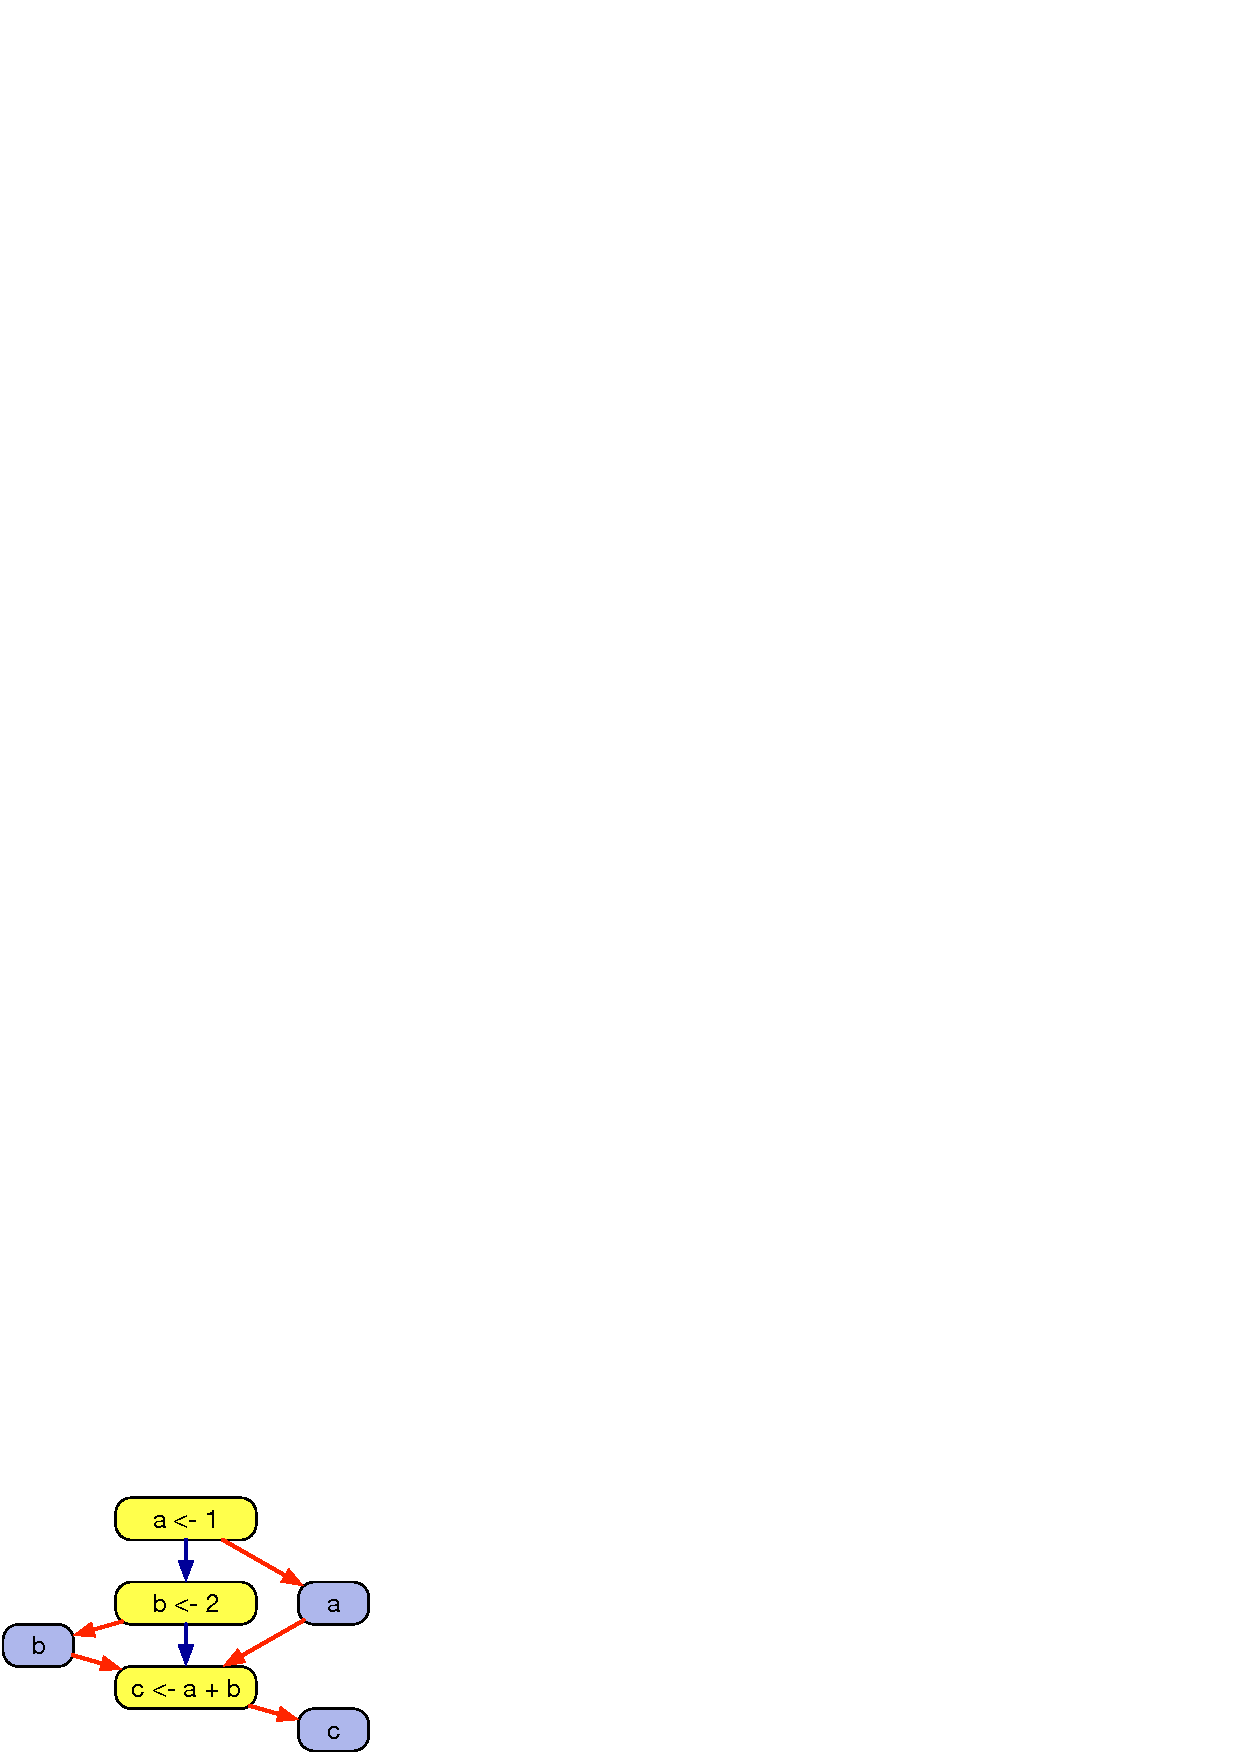
\includegraphics[width=0.3\textwidth]{figures/simple-graph.png}
%    \caption{A simple R script's provenance graph.}
%    \label{fig:simple-graph}
%\end{figure}

We associate three types of information with provenance:  environment information, coarse-grained information, and fine-grained information. \dfn{Environment information} includes information about the computing environment in which the script was executed.  This includes information such as the operating system version, the R version, and the versions of the R libraries used, as each of these may play a role in understanding the details of how a script behaves.  \dfn{Coarse-grained information} includes the source code of the script(s), the data input to the script, the data output by the script, and plots produced by the script.  \dfn{Fine-grained information} includes an execution trace.  Specifically, for each line of the script that is executed, fine-grained information includes the data used on that line and any data computed by, or object created by, that line.  Our E2ETools can use this fine-grained information to help a user understand exactly how any data value or object in the script was computed or derived. 
%as shown graphically in the simple example in \autoref{fig:simple-graph}.

\bigskip
\noindent
%\noteae{I've removed (commented out) the ``Motivating example''. If we include one (i.e., a real-life example), we should work through it with our tools. Otherwise, we can make the same points with the straightforward examples that are already set up below}

%\section{Motivating Example}

%Kim has been studying blah blah and has a growing suspicion that there is a relationship between x and y.  She has found a reliable source of data and has developed an R script to analyze the data. While discussing this with her colleague Fred over lunch, he tells her about another good source of data for her study.  \notebl{Obviously, need something other than blah blah and x and y.} \noteae{we could put it in a Bayesian context, where Kim is using an uninformative (flat) prior and Fred points her at another dataset that could sharpen (inform) her prior.}

%Excited by this new opportunity, she downloads the data and tries to load them into her script.  Unfortunately, the data are not stored in the same way, and contain extra information she does not need \noteae{this equates/conflates data with dataset. Intentional? Standard usage? From the prov perspective, they are both objects...and that is pointed out in the ``What is data provenance'' section, below}.  With some effort, she is able to modify her script so that it can read both datasets and combine them in such a way that her script can analyze them.

%Things seem to be going well.  She continues to work on her analysis and modifies her script to produce a plot showing the relationship.  With the first dataset there seemed to be a strong relationship between x and y, but with the addition of the second dataset, it's not clear there is a relationship at all.  Why have the results changed? 
%\noteae{nothing has ``gone wrong'' unless Kim was so wedded to her preconceived notion about the hypothesis implied by the relationship in her data, or so convinced that her self-worth is tied up in a \textit{P} value that she is not open to new information. }

%Fortunately, Kim used rdtLite to collect data provenance as she was working on her script.  She starts up provDebugR to examine the calculations the script had done, thankful that the provenance-based debugger allows her to examine the data values after the time-consuming downloading and cleaning steps instead of needing to rerun her script from the beginning to see these intermediate values.  Doing this, she realizes that the values in the second dataset are much lower than those of the first dataset.  She goes back to the website from which she downloaded the second dataset to get a better understanding of how they collected their data.  As she examines their methodology, she finds the problem.  They used different units than in the first dataset.  Returning to her script, she adds the instructions to do the necessary conversion and now the second dataset corroborates the results of the first dataset. 
%\noteae{lucky her. in the real world, most second datasets fail to support the first. Hence the 's ``reproducibility crisis''}.

%\noteae{more seriously, though. The point of our tools is that they collect the prov silently so that Kim doesn't need to have had the foresight to collect the provenance. She just needs to use the tools, which have been collecting prov for her.}

%With the positive results in hand, Kim writes a paper, being careful to save the script, data, and data provenance so that she will be certain to be able to address any questions the reviewers may have.  After several months, Kim hears from the reviewers.  The reviews are quite positive, however, the reviewers have requested that the plots be presented differently.

%Kim pulls up the saved script and begins making the requested changes.  Unfortunately, things do not go smoothly.  With the passage of time, Kim has forgotten how the script works and wishes she had done a better job of commenting and cleaning up the script.  Now, she gets an inscrutable error just trying to rerun the code.  She is still using the same data and the same script.  Why doesn't it work? 
%\noteae{but she had the foresight to collect prov (above) so why didn't it help her here? Seems forced. If she were using provtools that collect the prov silently, this would be moot} \notebl{Collecting provenance is different than saving the environment}

%Kim uses provExplainR to compare the data provenance from when she submitted the paper to the data provenance of the current failed execution.  In doing this she discovers that she is running a different version of R and that she has downloaded a new version of one of the packages she is using. Could one of these be the cause of her problems?  Looking more closely at the error, she sees that it is coming from a call to a function in the recently updated package.  Using provDebugR's StackOverflow feature, she quickly learns how other users have resolved the error she is getting.  Fortunately, this turns out to be easy to fix and Kim gets her script running again.

%In this example, we have shown data provenance as providing a foundation that tools can use to help a programmer understand the behavior of their scripts.  In the remainder of the paper, we elaborate on what we mean by data provenance and the tools that we provide to collect and use provenance for R scripts.

\section{A first example}

Consider this simple example, \file{mtcars\_example.R}, that loads in the \samp{cars} dataset and plots miles per gallon (\code{mpg}) as a function of the number of cylinders (\code{cylinders}) (\autoref{listing:car}).

%\noteeb{I modified the script slightly so it matches the provenance summary and so we don't have to explain Rdata.rds.}

%\lstinputlisting[float=t,language=R, style=mystyle, caption={Source code for mtcars\_example.R.  This code is used to demonstrate the lineage traces provided by the debug.lineage function as described in the text}, label=listing:car]{./examples/mtcars_example.R}

\begin{figure}[t]
\begin{example}
# Load the mtcars data set that comes with R
data(mtcars)

# All the cars
allCars.df <- mtcars

# Create separate data frames for each number of cylinders
cars4Cyl.df <- allCars.df[allCars.df$cyl == 4, ]
cars6Cyl.df <- allCars.df[allCars.df$cyl == 6, ]
cars8Cyl.df <- allCars.df[allCars.df$cyl == 8, ]

# Create a table with the average mpg for each # cylinders
cylinders = c(4, 6, 8)
mpg = c(mean(cars4Cyl.df$mpg), mean(cars6Cyl.df$mpg), mean(cars8Cyl.df$mpg))
cyl.vs.mpg.df <- data.frame (cylinders, mpg)

# Plot it
plot(cylinders, mpg)
\end{example}
\caption{Source code for mtcars\_example.R.  This code is used to demonstrate the lineage traces provided by the debug.lineage function as described in the text.}
\label{listing:car}
\end{figure}

%The following commands (\autoref{listing:car-summarize}) run the script, collect its provenance, and produce a textual summary of the provenance (\autoref{listing:car-summarize-output}).
%\lstinputlisting[float=h,language=R, style=mystyle, caption={Collect and summarize provenance}, label=listing:car-summarize]{./code/car-summarize.R}

The following commands run the script, collect its provenance, and produce a textual summary of the provenance.
\begin{example}
library(rdtLite)
prov.run("mtcars_example.R")
prov.summarize()
\end{example}

%\lstinputlisting[float=h, style=mystyle, caption={Provenance summary for mtcars\_example.R, showing the environment in which the script was executed, identifying the script, input and output files, and any errors or warnings encountered when the script was executed.}, label=listing:car-summarize-output]{./code/prov-summary.txt}

\begin{figure}[htbp]
    \begin{example}
PROVENANCE SUMMARY for mtcars_example.R

ENVIRONMENT:
Executed at 2022-07-28T13.52.25EDT
Total execution time was 1.516 seconds
Script last modified at 2022-07-22T10.41.25EDT
Executed with R version 4.2.1 (2022-06-23)
Platform was x86_64, darwin17.0
Operating system was macOS Catalina 10.15.7
User interface was 2022.02.3+492 Prairie Trillium (desktop)
Document converter was 2.2.1 @ /usr/local/bin/pandoc
Provenance was collected with rdtLite1.4
Provenance is stored in /Users/blerner/tmp/prov/prov_mtcars_example
Hash algorithm is md5

LIBRARIES (loaded by script):
None (see notes below)

SCRIPTS:
1[:] /Users/blerner/Documents/Process/DataProvenance/Papers/RJournal/scripts/
    examples/mtcars_example.R

PRE-EXISTING:
None

INPUTS:
1[:] /Library/Frameworks/R.framework/Versions/4.2/Resources/library/datasets/
    data/Rdata.rds

OUTPUTS:
1[-] /Users/blerner/Documents/Process/DataProvenance/Papers/RJournal/scripts/
    dev.off.11.pdf

CONSOLE:
None

ERRORS & WARNINGS:
None

NOTES: Files are listed in the order of execution (script 1 = main script).
The status of each file in its original location is marked as follows:
File unchanged [:], File changed [+], File missing [-], Not checked [ ].
Copies of original files are available on the provenance directory.

Libraries loaded by the user's script at the time of execution are displayed.
Note that some libraries may have been loaded before execution. Use details = 
TRUE to see all loaded libraries along with script, file, and message details.
    \end{example}
    \caption{Provenance summary for mtcars\_example.R, showing the environment in which the script was executed, identifying the script, input and output files, and any errors or warnings encountered when the script was executed.}
    \label{listing:car-summarize-output}
\end{figure}

%\begin{figure}
%\begin{verbatim}
%ENVIRONMENT:
%Executed at 2020-05-04T14.55.52EDT 
%Total execution time is 2.018 seconds
%Script last modified at 2020-05-04T14.51.41EDT 
%Executed with R version 3.6.0 (2019-04-26) 
%Executed on x86_64 running darwin15.6.0 
%Provenance was collected with rdtLite 1.2.1 
%Provenance is stored in /Users/blerner/provenance/prov_mtcars_example 
%Hash algorithm is md5 

%LIBRARIES:
%base 3.6.0
%datasets 3.6.0
%ggplot2 3.1.1
%graphics 3.6.0
%grDevices 3.6.0
%methods 3.6.0
%rdtLite 1.2.1
%stats 3.6.0
%utils 3.6.0
%\end{verbatim}
    %\caption{Provenance environment information for mtcars\_example.R %\notetp{should this be a listing too?}}
    %\label{fig:env}
%\end{figure}
%\notemis{Why don't we include in Figure 1 the complete output of prov.summarize()? I am worried that it will be confusing if we show the call to prov summarize, discuss some of the coarse grain information, but don't include it in the listing.}

The provenance summary is shown in \autoref{listing:car-summarize-output}.
The environment information (lines 3--18) reports details of the computing environment in which the script was executed, such as the processor and operating system on which it ran and the version of R and R libraries used. The coarse-grained information (lines 20--36) identifies the location in the file system of the script, the input dataset, and the plot produced.  The fine-grained information, which is not displayed by \code{prov.summarize()} but is accessible via other tools, indicates the input and output data for each line of code executed, linking them together so that one can see how the values computed in one statement are used in later statements.
For example, the provenance debugger can use fine-grained information to display everything that is derived from a variable.  
\begin{example}
library(provDebugR)
prov.debug()
debug.lineage("cars4Cyl.df", forward = TRUE)
\end{example}

%the following lines of  code (\autoref{listing:car-lineage}) use our provenance debugger and the fine-grained information to show everything that is derived from \code{cars4Cyl.df}. 
The resulting output 
%(\autoref{listing:car-lineage-output}) 
displays the line numbers and code for everything computed, either directly or indirectly, from \code{cars4Cyl.df} .
\begin{verbatim}
Var cars4Cyl.df 
	8: 	  cars4Cyl.df <- allCars.df[allCars.df$cyl == 4, ] 
	14: 	 mpg = c(mean(cars4Cyl.df$mpg), mean(cars6Cyl.df ...
	15: 	 cyl.vs.mpg.df <- data.frame (cylinders, mpg) 
	18: 	 plot(cylinders, mpg) 
	NA: 	 mtcars_example.R 
\end{verbatim}

%\lstinputlisting[float=h,language=R, style=mystyle, caption={Show forward lineage of cars4Cyl.df}, label=listing:car-lineage]{./code/car-lineage.R}

%\lstinputlisting[float=h,language=R, style=mystyle, caption={Forward lineage of cars4Cyl.df}, label=listing:car-lineage-output]{./code/car-lineage-output.R}

Alternatively, a modified version of the same command 
%(\autoref{listing:car-lineage2}) 
\begin{example}
debug.lineage("cars4Cyl.df")
\end{example}
shows the lines of code that lead to the value for \code{cars4Cyl.df} being computed.
%(\autoref{listing:car-lineage2-output}).
\begin{verbatim}
Var cars4Cyl.df 
	2: 	 data(mtcars) 
	5: 	 allCars.df <- mtcars 
	8: 	 cars4Cyl.df <- allCars.df[allCars.df$cyl == 4, ] 
\end{verbatim}

%\lstinputlisting[float=h,language=R, style=mystyle, caption={Show backward lineage of cars4Cyl.df}, label=listing:car-lineage2]{./code/car-lineage2.R}

%\lstinputlisting[float=h,language=R, style=mystyle, caption={Backward lineage of cars4Cyl.df}, label=listing:car-lineage2-output]{./code/car-lineage2-output.R}

%An individual datum or a set of data could be ``raw'' (collected by an individual or an automated sensor) or ``derived'' (computed or estimated from the raw data). For either raw or derived data, provenance would include when and where the data were collected or derived; and by what people, instruments, sensors, or post-processing software. Our focus with ProvTools is the collection and use of language-level provenance for data that is created by R scripts. \notemis{I just had someone review our ProvBuild paper and she pointed out that when people see provenance, those who have heard the term most often think of database provenance. I've switched to introducing work like this as "language-level provenance" and then just using "provenance" after that. I might also call the data "original" rather than raw. Some devices (or people) will transform the data in ways before recording it; the key differentiator is that there is no way to get it back if you lose it; derived data can, in theory, be recomputed; raw data cannot.}


%\noteae{Why call out sensors? Wouldn't you would want to know the same thing for data collected by a person. I've revised that a bit.}

%The provenance of derived data depends upon the computing environment, the input data, and the script(s) that did the computation. We refer to these three items together as ``coarse-grained'' provenance. Coarse-grained provenance can provide useful documentation of the origins of the data and may help with reproducibility. \notemis{I think "file-level" is a dangerous name to use here; again, those who know about provenance will think of file system provenance. We could just call it coarse-grained?" Also might it not be helpful to ground this discussion with examples of provenance?}

%We are also interested in ``fine-grained'' provenance, which augments coarse-grained provenance with an execution trace through the script and any intermediate data values created by the script. The more detailed understanding of the data provided by fine-grained provenance can be helpful when debugging or cleaning the script.

%\notetp{I think the reader need a concrete example at some point.}

%\notebl{I have commented out the entire Use cases section as it seems we have already hit on all the points in the earlier example.  It's still in the Latex file if anyone wants to see it.}

% \section{Use cases}
% Collecting fine-grained data provenance is a challenging task, but it has little benefit if the provenance is never used.  In this section, we describe various ways that provenance can be used to help the scientist or data analyst with their job. \notemis{Use cases are typically specific things a user wants to do, not broad categories ; the walkthrough example should allow us to describe things that a user wants to do with the script in question and then generate the categories of the types of things users do. Alternately, you can say that these are categories and then translate them to use cases.}

% \noteae{I assume that file-level provenance also has little benefit if it is never used. Will we have use cases for both file level and fine-grained provenance?}

% \notemis{I recommend constructing a simple example that we can use to demonstrate all the use cases -- it should be something real-ish, but small enough to present both the script and meaningful provenance snippets.}

% \noteeb{I like the use case of trying to verify a published result. Suppose we come across an interesting paper and the author has archived his or her data, R script, and provenance. We want to verify the author's results, so we first use provSummarizeR to make sure we have access to all of the original inputs and are aware of any differences in computing environment. We run the script and get a different result. So then we use provExplainR to explore the differences more closely. Perhaps the version of R or of one of the R libraries is different. Or maybe the input files are not the same or the data retrieved from a URL has changed. If provExlainR identifies differences in the provenance graphs, we use provDebugR to look more closely at intermediate data values and steps executed at the point where the graphs begin to diverge.  We could also use provViz to see how the execution pathways might diverge at that point.}

% \subsection{Documentation}
% \notemis{I think this is conflating two things: documentation which should precisely mirror the definition used in the rest of the world and program comprehension, which is a term used to describe understanding what a program is doing at a somewhat deeper level.}
% \noteae{this subsection comes sort of out of nowhere. Could use a better transition from something. Maybe it belongs in the ``what is data provenance'' section, above}
% Fundamentally, data provenance is documentation.  What data were used as input?  What script was used to process the input?  What version of R and user-contributed packages were used to interpret the script?  On what computing platform?  Just as with the provenance of a piece of art, the purpose of documentation at this level is to build trust.  You wouldn't buy a used car without checking its Carfax report.  Data provenance is essentially the Carfax report for data.  The provSummarizeR tool described below provides this type of report.
% \notetp{Bad cultural expectation. I don't think anyone outside of the US knows Carfax. This sort of things should be avoided.}
% \noteae{yep}

% \subsection{Debugging}
% \noteae{ditto here. I'm not following the organization of the subsections under the Use cases section. However, this one seems like if we included a use-case it could fit well here}
% Given fine-grained provenance, it is possible to examine the values of variables in a script at different points during execution.  This can help a data analyst track down errors in the script's execution.

% In addition, fine-grained provenance allows the data analyst to ask the questions "how did \textit{x} get its value?" and "what was computed based on the value of \textit{x}?"  In this way, the analyst can focus in on the portions of the script that are relevant to a specific computation. \noteae{is this referring to ProvClean?}
% \noteeb{provDebugR and provViz}

% We provide the provViz tool described below to allow a graphical examination of the fine-grained provenance.  The provDebugR tool, under development, provides a more standard command-line debugger interface to the same information.

% \subsection{Reproducibility}
% A reproducible script is one that can be re-executed and get the same results.  Unfortunately, this is surprisingly difficult.  With the passage of time, new libraries may be installed which break the script.  If you share your script with a colleague, it might not behave the same.  The provExplainR tool, described below, can be used to understand what has changed.  It compares the provenance collected by two executions of a script and identifies differences in the computing environment, input data, and scripts to help the data analyst understand why a script is no longer working.

% Scripts are often developed in an exploratory fashion.  When complete, the data analyst may realize that only some of the plots being produced are useful.  The provClean tool, under development, uses provenance to determine which code was used to produce the desired output and retain just that code.

% \noteeb{We might expand on this with the example of someone trying to reproduce a result published by someone else (see above). This is (or should be) a fairly common scenario. How would provenance and our tools make this easier? Why might it fail?} 

%In future work, we plan to build a tool that uses provenance to create a virtual machine that encapsulates the computing environment with the script and data to facilitate re-running the script.

%{\bf Encapsulation: should we include this.  Nobody is maintaining it.}

Having seen an introductory example of some things the E2ETools can do, we
now turn to a more detailed discussion of each tool.

\section{The end-to-end provenance tools}

%\noteae{From here on down, the paper reads pretty cleanly}

The E2ETools consist of three types of packages: 
\begin{itemize}
    \item A package to collect provenance: \CRANpkg{rdtLite};
    \item Packages that process data provenance to provide information to the user about a particular script and its execution:  \CRANpkg{provSummarizeR}, \CRANpkg{provDebugR}, \CRANpkg{provViz}, and \CRANpkg{provExplainR};
    \item Packages to enable tool developers to more easily use data provenance:  \CRANpkg{provParseR} and \CRANpkg{provGraphR}.
\end{itemize}

%provSummarizer provides a human-readable summary of the provenance.  provDebugR allows debugging of R code going backward and forward through the code without rerunning.  
%provClean can reduce a complicated script to the minimal code necessary to produce a particular output.
%provViz allows examination of the provenance via a graphical representation of the execution trace.

%There are two packages intended for tool developers:  provParseR and provGraphR.  provParseR reads in the provenance and provides an API for convenient access to parts of the provenance.  provGraphR provides an API to answer lineage questions about the collected provenance.

We describe each of these packages, beginning with provenance collection.  All the tools described are available on CRAN.

%\notemis{Since this is just an overview, I wonder if it might better be captured in a table; then we just say, "Table 1 lists all the tools that comprise the <Name> suite." Second, calling this the rdtLite is, I think, confusing -- you've mentioned ProvTools above, rdtLite not at all. If the package is provtools, then that's what this section should be; it then relies on Rdt and Rdtlite as its capture mechanism}

\subsection{Collecting provenance with rdtLite}

The rdtLite package collects provenance from R scripts as they execute.\footnote{rdtLite is a simplified version of RDataTracker \citep{Lerner:TAPP14, Lerner:Informatics}.}
rdtLite captures provenance data from both scripts and interactive console sessions. To capture provenance for a script, the user runs the script using the \code{prov.run} function.
%rdt is available on github (https://github.com/End-to-end-provenance/rdt).  rdtLite is more stable but collects less detailed provenance than rdt does.  The additional provenance collected by rdt includes fine-grained provenance internal to functions and internal to control constructs.  Both tools output their provenance using the same PROV-JSON format.

%(\autoref{listing:rdtlite}) 
\begin{example}
library(rdtLite)
prov.run("script.R")
\end{example}
To collect provenance for an interactive session, the user begins the session with the \code{prov.init} function and concludes it with \code{prov.quit}. 
%(\autoref{listing:interactive})
\begin{example}
library(rdtLite)
prov.init()
data <- read.csv("mydata.csv")
plot(data$x, data$y)
prov.quit()
\end{example}

%\lstinputlisting[float=h,language=R, style=mystyle, caption={Run a script and capture provenance}, label=listing:rdtlite]{./code/rdtlite.R}

%\lstinputlisting[float=h,language=R, style=mystyle, caption={Capture provenance in a console session}, label=listing:interactive]{./code/interactive.R}

rdtLite collects information about each file or URL read by the script, each file written by the script, and each plot created by the script.  In addition, it records an execution trace of the top-level R statements.  This trace identifies the statement executed.  It records any variables set or used by the statement.  When a variable is set, it records the type of the value, including its container (such as vector, data frame, etc.), dimensions, and class (e.g., character, numeric).  If the container is a vector of length 1, rdtLite records its  data value, embedded in the provenance (which is stored in a JSON file).  rdtLite can save the values of larger containers in separate snapshot files.  The user controls how much data to save using the \code{snapshot.size} parameter in \code{prov.init} and \code{prov.run}.  The default is to not save snapshots. rdtLite also records any warning or error messages generated when the statement is executed.  To capture similar information about scripts that are included using the \code{source} function, calls to \code{source} must be replaced with calls to \code{prov.source}.

The provenance is stored in a JSON file using a format
that extends the PROV-JSON standard \citep{provjson}.\footnote{\url{https://github.com/End-to-end-provenance/ExtendedProvJson/blob/master/JSON-format.md}.} The extended format provides structured information about fine-grained provenance, such as a list of libraries used, a mapping from functions called to the libraries from which they came, script line numbers, and data values and their types.  More 
information about the extended JSON format is provided in the \hyperlink{sec:ExtendedJSON}{Appendix}.

The JSON file is stored in a provenance directory that also contains copies of all input and output files and the R scripts executed.  By default, the provenance data is stored in the R session temporary directory, but the user can change this location either at the time that \code{prov.run} or \code{prov.init} is called or by setting the \code{prov.dir} option, for example, in the .Rprofile file.

%\notemis{This feels like a pretty low level detail for inclusion here; it reads more like documentation. It interferes with the flow of the narrative; I'd vote for removing it.}
%If an R script calls R's \texttt{source} function to execute another R script, calls to \texttt{source} should be replaced with calls to rdtLite's \texttt{prov.source} function.  This allows provenance collection to continue within the sourced script.  If \texttt{prov.source} is not used, the call to the \texttt{source} function appears as a single statement in the execution trace, and uses of variables or updates to variables within the sourced script are not recorded.

Upon completion of a script called with \code{prov.run}, or after a call to \code{prov.quit}, rtdLite creates and populates a directory named either \samp{prov\_script}, where \samp{script} is the name of the script file, or \samp{prov\_console} for an interactive session.
The directory will contain:
\begin{itemize}
    \item \file{prov.json} - the JSON file containing the fine-grained provenance
    \item \file{data} - a directory containing copies of input and output files, URLs, plots created, and snapshot files.
    \item \file{scripts} - a directory containing a copy of the scripts for which provenance was collected.%\notemis{I changed this assuming we remove the paragraph above; if we decide not to, then I think this still works.}
\end{itemize}

The rdtLite default is to overwrite this information if the same script is executed again or if \code{prov.init} is used again in a console session. However if the \code{overwrite} parameter is set to FALSE, the provenance is stored in a unique, time-stamped directory, allowing provenance from multiple executions to be analyzed and compared.

\subsection{Using provenance}
Having the provenance is extremely valuable, but it is not particularly usable without tools that read the provenance and provide \emph{information} or enable \emph{reproducibility}.  We next describe four tools that use provenance to help R programmers understand executions of their script.  The \CRANpkg{provSummarizeR} package provides a concise textual summary of an execution.  The \CRANpkg{provViz} package provides a graphical visualization of the provenance.  The \CRANpkg{provDebugR} package uses collected provenance to help programmers debug their code.  The \CRANpkg{provExplainR} package compares provenance from two executions to help the programmer understand changes between them. These applications exist in packages separate from \CRANpkg{rdtLite} and would work equally well with provenance collected by other tools that produce the same JSON format.  

%\noteeb{Suggest reordering tools as follows: provSummarizeR (already demonstrated and simplest), provViz (bird's eye view of provenance), provDebug R, provExplainR (both use detailed provenance). This is the order in the abstract.}

%\noteae{I agree with Emery's suggestion for re-ordering, which also addresses Margo's later comment on provSummarizeR}

\subsubsection{provSummarizeR}

The purpose of \CRANpkg{provSummarizeR} is to produce a concise record of the environment in which a script was executed.  This information could be particularly valuable when including a script and its results in a paper, or when sharing a script with a colleague. For an example, please see \autoref{listing:car-summarize-output} above. The summary includes the following information:

%For example, consider the following simple script:
%\lstinputlisting[float=h,language=R, style=mystyle, caption={\notetp{TODO}}, label=listing:summarize]{./code/summarize.R}

% \begin{itemize}
%     \item a description of the execution environment, 
%     \item a list of the libraries used and their versions,
%     \item a list of any scripts source'd,
%     \item a list of the input and output files, including their timestamp and hash value
%     \item a list of the errors and warnings encountered, including the message and the line on which the error occurred
% \end{itemize}

%For example, consider this simple R script:

% \begin{verbatim}
% data <- read.csv ("mydata.csv")
% plot (data$x, data$y)
% \end{verbatim}

%The summary of the provenance generated by this short script is shown below.

%\notebl{Looking for suggestions of how to format this so it looks better.}
%\notetp{I suggest to use listings, there is line numbers and things can be referred to in the text. I am happy to do the switch if that helps.}

%\hrule

%\begin{verbatim}
%PROVENANCE SUMMARY for script.R 
%\end{verbatim}
%\notemis{It's not obvious that the first block of text is describing what appears below and is not actually part of the summary; listing formats typically allow comments, which is what I think we probably want here. More fundamentally, we actually show half of a summary at the very beginning; why not just do that fully and skip it here? We could just refer back to the initial example and give some of the options here; right now the discussion is split and it looks accidental, because neither section refers to the other.}
%\notetp{This one will be easier if I get the raw output to put in the listing.}
%\begin{quote}

\begin{itemize}
\item The ENVIRONMENT section shows information about when the script was modified and executed, what version of R was used, what hardware and operating system were used, what R environment (such as RStudio) was used, what tool collected the provenance, where the provenance is stored, and what hash algorithm was used to store hash values for files used in the input and output of the script.
%\end{quote}

%\begin{verbatim}
%ENVIRONMENT:
%Executed at 2018-12-07T14.29.59EST 
%Script last modified at 2018-12-03T13.49.29EST 
%Executed with R version 3.5.1 (2018-07-02) 
%Executed on x86_64 running darwin15.6.0 
%Provenance was collected with rdtLite 1.0.3 
%Provenance is stored in ~/tmp/prov/prov_script 
%Hash algorithm is md5 
%\end{verbatim}

%\begin{quote}
\item The LIBRARIES section shows the libraries loaded by the script and their version numbers.
%\end{quote}
%\begin{verbatim}
%LIBRARIES:
%base 3.5.1
%datasets 3.5.1
%ggplot2 3.0.0
%graphics 3.5.1
%grDevices 3.5.1
%methods 3.5.1
%provSummarizeR 1.0
%stats 3.5.1
%utils 3.5.1
%\end{verbatim}

%\begin{quote}
\item The SCRIPTS section lists the main script and any scripts that are included in the execution of this script using the \code{source} or \code{prov.source} functions.
%\end{quote}
%\begin{verbatim}
%SOURCED SCRIPTS:
%None
%\end{verbatim}

%\begin{quote}
\item The PRE-EXISTING section shows any variables where the script uses a value that was bound to the variable before the script started.  This is a common R programming error that can lead to unexpected results if the script is run again in a different environment, where such a variable might have a different value or not be set at all.
%\end{quote}
%\begin{verbatim}
%PRE-EXISTING:
%None
%\end{verbatim}
%\begin{quote}
\item The INPUTS and OUTPUTS sections list all input and output files, the date they were last modified, and their hash values, using the hash algorithm shown in the environment section.
%\end{quote}
%\begin{verbatim}
%INPUTS: 
%File : mydata.csv 
%   2018-12-03 13:50:14 
%   f777f89d9b76dfda566ea85d24a391e1 

%OUTPUTS: 
%File : dev.off.4.pdf 
%   2018-12-07 14:30:00  
%   c90d4198fd8e59f7f92a2e69ed5c3701 
%\end{verbatim}

\item The CONSOLE section shows any output sent to the console when the script executed.

%\begin{quote}
\item The ERRORS \& WARNINGS section lists any errors or warnings that occurred when the script executed, including the number of the line that caused them.
\end{itemize}

%\end{quote}
%\begin{verbatim}
%ERRORS:
%None
%\end{verbatim}

%\hrule
In our own day-to-day work, we use \CRANpkg{provSummarizeR} to document the processing of real-time meteorological and hydrological data at Harvard Forest. Data and plots of data captured in the past 30 days, including air temperature, precipitation, stream discharge, and water temperature, are updated and posted every 15 minutes.\footnote{\url{https://harvardforest.fas.harvard.edu/met-hydro-stations}} Also posted at the same site are provenance summaries for the script execution that creates the plots.

There are three functions provided to generate summaries:
%(\autoref{listing:summarize2})
\begin{example}
prov.summarize(details = FALSE)
prov.summarize.file(prov.file, details = FALSE)
prov.summarize.run(r.script, details = FALSE)
\end{example}
\begin{itemize}
\item \code{prov.summarize} produces a summary for the last provenance collected in the current R session.
\item \code{prov.summarize.file} takes the name of a JSON file containing provenance and produces a summary from it.
\item \code{prov.summarize.run} takes the name of a file containing an R script.  It runs the script, collects its provenance, and produces a summary.\footnote{All three functions have additional optional parameters.  For details, see the online help page.}
\end{itemize}

By passing \code{TRUE} for the \code{details} parameter, the user can see more detail about some aspects of the provenance.  In particular, 
\begin{itemize}
    \item The libraries section is divided into three parts.  The first part shows the libraries loaded by the script.  The second part shows the libraries that were loaded before the script starts.  The third part shows the libraries loaded by the rdtLite code itself.  
    \item The information about script, inputs, and output files includes modification date and hash value.
    \item The information about errors and warnings includes the line number on which each occurred.
\end{itemize}

%\lstinputlisting[float=h,language=R, style=mystyle, caption={Three versions of prov.summarize}, label=listing:summarize2]{./code/summarize2.R}

%If the optional parameter \code{save} is \code{TRUE}, the summary will be saved to a file in the provenance directory in addition to being displayed on the screen.  If the optional parameter \code{create.zip} is set to \code{TRUE}, the provenance directory will be packaged into a zip file.

%\texttt{provSummarizeR} is available on CRAN.

The provViz and provDebugR tools described below provide a similar set of three functions: one to use the last provenance collected, one to use a specific JSON file, and one to run a script and use its provenance.

\subsubsection{provViz}

\begin{figure}[p]
    \centering
%    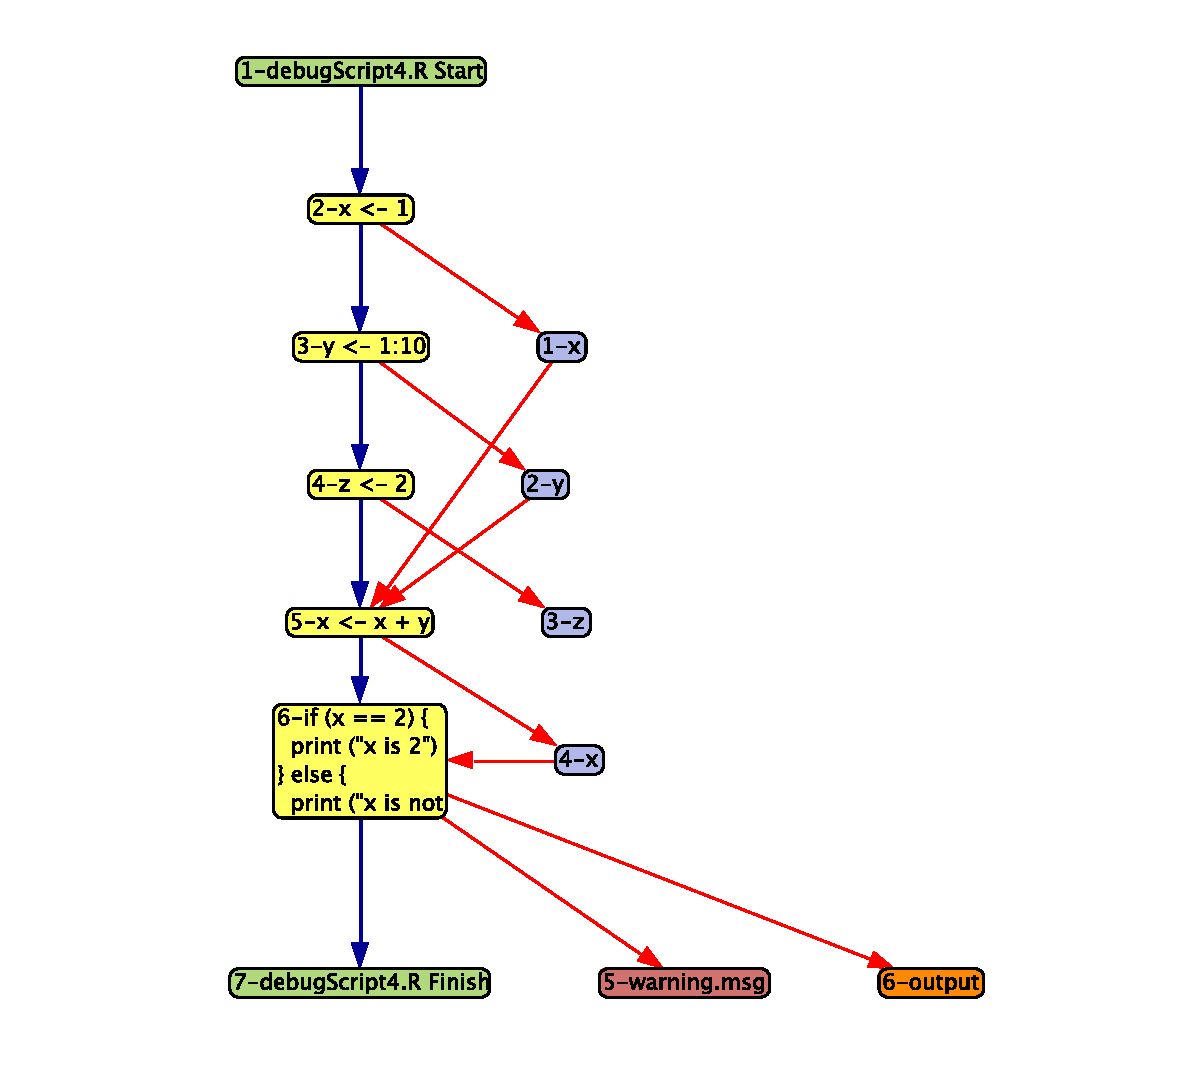
\includegraphics[width=\textwidth]{figures/debugScript4.eps}
    \includegraphics[width=.75\textwidth]{figures/car-graph.pdf}
    \caption{A provenance graph as displayed using \CRANpkg{provViz}.  Yellow nodes represent statements in the code, blue nodes represent variables, orange nodes represent files and green nodes mark the start and end of the script.}
    \label{fig:visualization}
\end{figure}

The \CRANpkg{provViz} package allows visual exploration of script execution as shown in \autoref{fig:visualization}.  There are two types of nodes: data nodes and procedure nodes.  Data nodes represent things such as variables, files, plots, and URLs.  Procedure nodes represent executed R statements.  An edge from a data node to a procedure node indicates that the statement represented by the procedure node uses the data represented by the data node. For example, the edge from data item, \samp{7-mpg}, to procedure node, \samp{9-plot(cylinders,mpg)}, indicates that \code{mpg} was used in the call to the \code{plot} function.
Conversely, an edge from a procedure node to a data node indicates that the procedure produced the data, for example, by assigning to a variable or writing to a file.  An edge between two procedure nodes represents control flow, indicating the order in which the statements were executed.

\CRANpkg{provViz} also allows the user to view the graph and explore it to examine intermediate data values or input and output files and to perform lineage queries.  The node colors indicate node type.  Data nodes representing variables are purple.  Files are tan.  Orange nodes represent standard output, while red data nodes represent warnings and errors.  Yellow nodes represent R statements.  Green nodes come in pairs and represent the start and end of a group of R statements. Clicking on a green node reduces the set of statements between the matching \samp{Start} and \samp{Finish} nodes into a single node, which is useful for making large graphs more manageable.

\begin{figure}[p]
    \centering
%    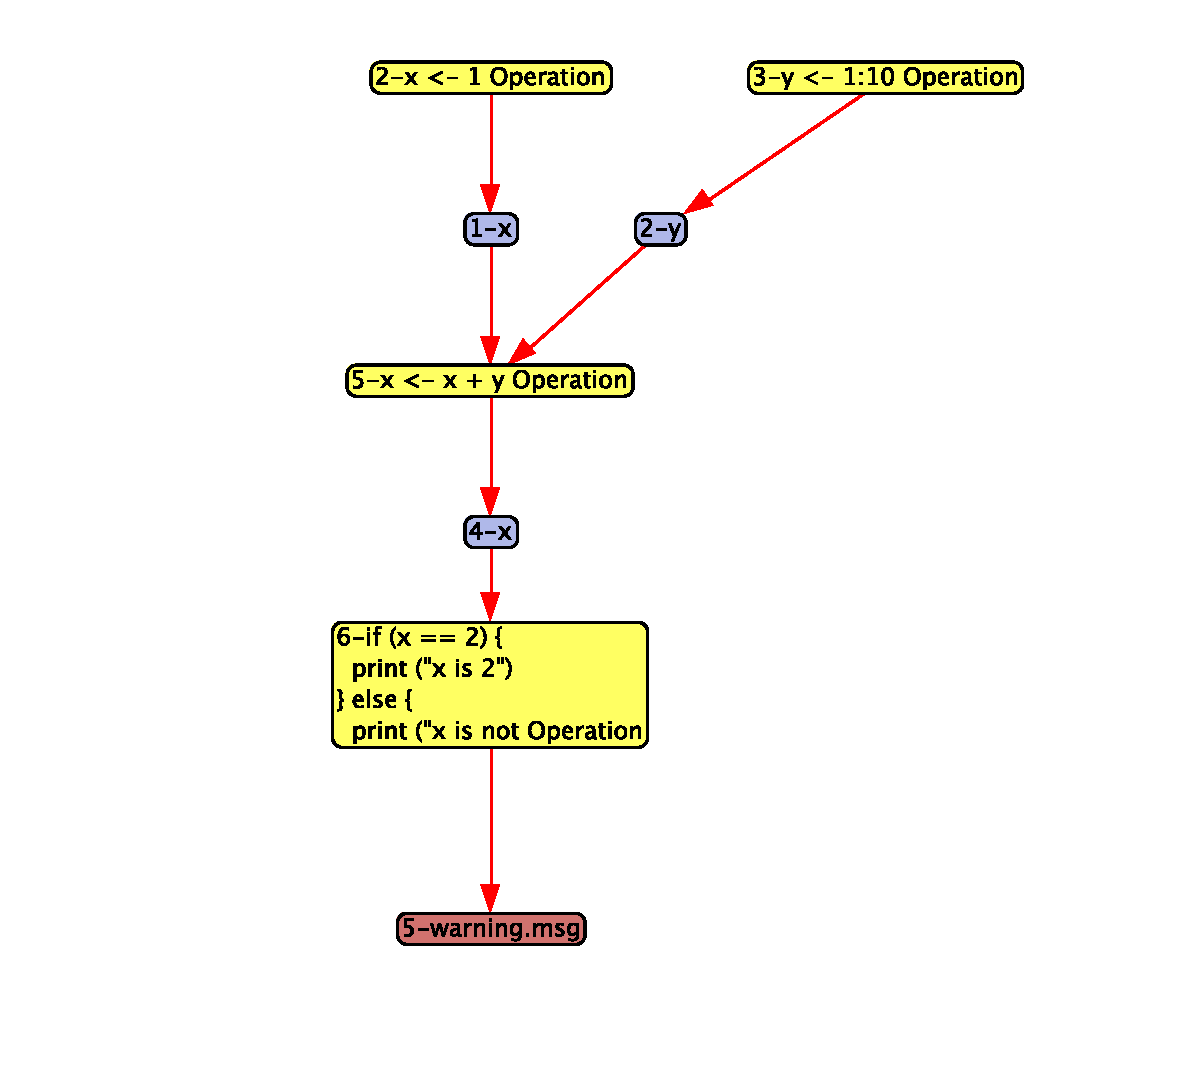
\includegraphics[width=\textwidth]{figures/debugScript4Lineage.eps}
    \includegraphics[width=.75\textwidth]{figures/car-lineage.pdf}
    \caption{Displaying the Lineage of 3-cars4Cyl.df}
    \label{fig:lineage}
\end{figure}

To see everything that depends on the value of a variable at a particular point in the execution of the script, the user can right-click on the data node and select \samp{Show what is computed using this value}.  This will display a subgraph containing just the data and procedure nodes that are in the lineage of the data node, as shown in \autoref{fig:lineage}, which shows the lineage of \samp{3-cars4Cyl.df}.  Notice that statements that do not use the value of \code{cars4Cyl.df}, either directly or indirectly, are not shown.

%Right-clicking on a warning or error node and selecting \samp{Show Message} displays the warning/error message produced by R.  To identify the computation leading up to the warning, the user can right-click on the warning message and select \samp{Show How Value was Computed}.  This will display a subgraph containing just the data and procedure nodes that are in the backward lineage of the warning node, as shown in \autoref{fig:lineage}.  As with \CRANpkg{provDebugR}, notice that the statement assigning to z is not included in the result.  Also, notice that the initial assignment to x and the assignment to y are not ordered as neither depends on the other.

In addition to examining data values and tracing lineages as in this example, provViz supports the following ways of exploring the provenance:

\begin{itemize}
    \item Viewing input and output data files
    \item Viewing plots created
    \item Viewing the source code for a node or the entire script
    \item Comparing R scripts
    \item Comparing provenance graphs
    \item Searching for nodes by name and type
    \item Sorting procedure nodes based on execution time
\end{itemize}

%The \texttt{provViz} package provides three functions:

%\begin{itemize}
%    \item \texttt{prov.visualize} displays the graph associated with the last provenance collected in the current R session.
%    \item \texttt{prov.visualize.file} reads the provenance from a file and displays its graph.
%    \item \texttt{prov.visualize.run} runs an R script, collecting its provenance, and displays the graph on completion of the script.
%\end{itemize}

%\noteeb{Most of our applications have these same three options (use last provenance in current session, use provenance from a file, or run script and use resulting provenance), so we might mention these at the beginning of this section instead of under each tool.}

provViZ itself is a small R program that connects to a Java program called DDG Explorer \citep{Lerner:IPAW14}, which does the actual work of creating and managing the display.  
%\texttt{provViz} is available on CRAN.

\subsubsection{provDebugR}

The \CRANpkg{provDebugR} package provides debugging support by using the provenance to help users understand the state of their script at any point during execution. It provides command-line debugging capabilities, but one could imagine building a GUI on top of these functions to produce a friendly interactive debugging environment. By using provenance, provDebugR provides insight into the entire execution and creates a rich debugging environment that provides execution context not typically available in debuggers.

For example, consider a simple, but buggy script.
%(\autoref{listing:bugged-script}).
\begin{example}
w <- 4:6
x <- 1:3
y <- 1:10
z <- w + y
y <- c('a', 'b', 'c')
xyz <- data.frame (x, y, z)
\end{example}
Running this script produces a warning and an error.
\begin{example}
Error in data.frame(x, y, z) : 
  arguments imply differing number of rows: 3, 10
In addition: Warning message:
In w + y : longer object length is not a multiple of shorter object length
\end{example}
%(\autoref{listing:error}).

%\lstinputlisting[float=h,language=R, style=mystyle, caption={Buggy script 1}, label=listing:bugged-script]{./code/bugged-script.R}

%\lstinputlisting[float=h, style=mystyle, caption={Errors and warnings from buggy script 1}, label=listing:error]{./code/error.R}

Of course, with a short script like this, a user could simply step through the script one line at a time and examine the results, but for the purposes of demonstrating the debugger, imagine that this code is buried within a large script.  The lines of code might not be consecutive as shown here, and it may even be difficult to determine what lines caused the reported errors.

%\notemis{It would make it much easier to read these examples if they were all clearly pulled out into figures so it was obvious where the examples start/end and where the prose starts/ends}

The debugger provides some functions that are particularly helpful for understanding warning and error messages.  For example, if the user needs help understanding where a warning came from, calling \code{debug.warning} with no arguments lists all the warnings; when called with a warning number, it displays the lines of code leading up to the warning.
%(\autoref{listing:debug-warning}).
\begin{example}
> debug.warning()
Possible results: 
                                                                              
1 In  w + y :  longer object length is not a multiple of shorter object length

Pass the corresponding numeric value to the function for info on that warning
> debug.warning(1)
Warning: In  w + y :  longer object length is not a multiple of shorter object length 
	1: 	 w <- 4:6 
	3: 	 y <- 1:10 
	4: 	 z <- w + y 
\end{example}
By omitting lines that do not contribute to the computations that lead to the warning, the R programmer should be able to find the problem more easily.

Similarly, the user can get information about what led up to an error using \code{debug.error}.
%(\autoref{listing:debug-error}).
\begin{example}
> debug.error()
Your Error: Error in data.frame(x, y, z): arguments imply differing number of rows: 3, 10

Code that led to error message:
	1: 	 w <- 4:6 
	2: 	 x <- 1:3 
	3: 	 y <- 1:10 
	4: 	 z <- w + y 
	5: 	 y <- c('a', 'b', 'c') 
	6: 	 xyz <- data.frame (x, y, z) 
\end{example}

%\lstinputlisting[float=h, style=mystyle, caption={Debugging warning messages}, label=listing:debug-warning]{./code/debug-warning.R}

%\lstinputlisting[float=h, style=mystyle, caption={Debugging error messages}, label=listing:debug-error]{./code/debug-error.R}

The \code{debug.error} function has an optional logical parameter, \code{stack.overflow}.  When set to \code{TRUE}, \code{debug.error} uses the stackexchange API to search Stack Overflow for posts about similar error messages.  
%To use the Stack Overflow API, the error message is first modified to remove references to quoted strings, as those represent things like variable names that are specific to the script.  It then uses Stack Exchange's API to search StackOverflow looking for posts that match the query, and sorts them by the number of votes they have received.
It lists the questions asked in the top six posts.  The user can select one and a tab will open in the user's browser displaying the selected post.

%\autoref{fig:error-trace}

\autoref{listing:stack-overflow} shows a sample dialog using \code{debug.error}.  Selecting 1 results in the user's browser going to the page displayed in \autoref{fig:stackoverflow}.\footnote{\url{    https://stackoverflow.com/questions/26147558/what-does-the-error-arguments-imply-differing-number-of-rows-x-y-mean}}  By scrolling down through answers to this question (not shown here), users will ideally obtain helpful information allowing them to solve their problem quickly.

%\lstinputlisting[float=t, style=mystyle-nonumber, caption={The output of a call to debug.error, showing the titles of posts on Stack Overflow related to the error encountered in the script.  The user can select an option to be taken to the corresponding Stack Overflow page.}, label=listing:stack-overflow]{./code/stack-overflow.R}

\begin{figure}[t]
\begin{example}
> debug.error(stack.overflow=TRUE)
Your Error: Error in data.frame(x, y, z): arguments imply differing number 
of rows: 3, 10

Code that led to error message:
1: 	 w <- 4:6 
2: 	 x <- 1:3 
3: 	 y <- 1:10 
4: 	 z <- w + y 
5: 	 y <- c('a', 'b', 'c') 
6: 	 xyz <- data.frame (x, y, z) 

Results from StackOverflow:
[1] "What does the error \"arguments imply differing number of rows: x, y\" 
    mean?"                                                 
[2] "ggplot gives \"arguments imply differing number of rows\" error in 
    geom_point while it isn't true - how to debug?"            
[3] "Checkpoint function error in R- arguments imply differing number of rows: 
    1, 38, 37"                                          
[4] "qdap check_spelling Error in checkForRemoteErrors(val) : one node 
    produced an error: arguments imply differing number of rows"
[5] "Creating and appending to data frame in R (Error: arguments imply 
    differing number of rows: 0, 1)"                            
[6] "Caret and GBM: task 1 failed - \"arguments imply differing number of rows\""                                                  

Choose a numeric value that matches your error the best or q to quit: 
\end{example}
\caption{The output of a call to debug.error, showing the titles of posts on Stack Overflow related to the error encountered in the script.  The user can select an option to be taken to the corresponding Stack Overflow page.}
\label{listing:stack-overflow}
\end{figure}

%\begin{figure}
%\begin{verbatim}
%> debug.error(stack.overflow = TRUE)
%Your Error: Error in data.frame(x, y, z): arguments imply differing number %of rows: 3, 10
%
%[1] "What does the error 'arguments imply differing number of rows: x, 
%y' mean?"                                         
%[2] "ggplot gives 'arguments imply differing number of rows' error in 
%geom_point while it isn't true - how to debug?"
%[3] "qdap check_spelling Error in checkForRemoteErrors(val) : one node 
%produced an error: arguments imply differing number of rows"
%[4] "Creating and appending to data frame in R (Error: arguments imply 
%differing number of rows: 0, 1)"                        
%[5] "Caret and GBM: task 1 failed - 'arguments imply differing number of 
%rows'"
%[6] "SparkR collect() and head() error for Spark DataFrame: arguments imply 
%differing number of rows"
%
%Choose a numeric value that matches your error the best or q to quit: 
%1
%\end{verbatim}
%\caption{Using \texttt{debug.error} \notetp{could be made a listing}}
%\label{fig:error-trace}
%\end{figure}

\begin{figure}[t]
    \centering
    \includegraphics[width=\textwidth]{figures/StackOverflow.png}
    \caption{Stack Overflow Page to Resolve an Error}
   \label{fig:stackoverflow}
\end{figure}

A common cause of programming errors in R is caused by automatic type conversions as occurs here:
\begin{example}
x <- 1
y <- 1:10
z <- 2
x <- x + y
if (x == 2) {
  print ("x is 2")
} else {
  print ("x is not 2")
}
\end{example}
Running this simple script 
%(\autoref{listing:error2}) 
produces this output.
%(\autoref{listing:warning2}).
\begin{example}
Error in if (x == 2) { : the condition has length > 1
\end{example}

%\lstinputlisting[float=h,language=R, style=mystyle, caption={Buggy script 2}, label=listing:error2]{./code/error2.R}

%\lstinputlhttps://www.overleaf.com/project/5c7b7d59b561ff3a7d3558a8isting[float=h, style=mystyle, caption={Warning from buggy script 2}, label=listing:warning2]{./code/warning2.R}

The programmer may be surprised or confused to get this warning message, as the assignment back to x may have been a mistake.  Since R is a dynamically-typed language, there is no error at the time of the assignment, but only later when the value is used.  The programmer can use \code{debug.variable} to quickly identify the type of x at each assignment 
%(\autoref{listing:debug-variable}). 
\begin{example}
> debug.variable(x, showType=TRUE)
Var: x 
	1: 	 1 	 x <- 1 
  container dimension type   
1 vector    1         numeric
	4: 	  2  3  4  5  6  7  8  9 10 11 	 x <- x + y 
  container dimension type   
2 vector    10        numeric
\end{example}
This shows that on line 4, x changed from a single element vector whose value was 1 to a 10-element vector containing the numbers 2 through 11.

%\lstinputlisting[float=h, style=mystyle, caption={Output from debug.variable}, label=listing:debug-variable]{./code/debug-variable.R}

Next, the programmer may want to find out why x became a vector.  The \code{debug.lineage} function provides this information.
%(\autoref{listing:debug-lineage}). 
\begin{example}
> debug.lineage(x)
Var x 
	1: 	 x <- 1 
	2: 	 y <- 1:10 
	4: 	 x <- x + y 
\end{example}
By showing the lines that led to  \code{x}'s value and type at line 4, we see the vector assignment to \code{y} in line 2, followed by the computation of \code{x} in line 4. Notice that line 3, the assignment to \code{z}, is not included in the lineage, since it played no role, either directly or indirectly in the value assigned to \code{x}.  Ideally, by examining the provenance, the programmer realizes that the assignment should have been to \code{y} rather than to \code{x}.

%\lstinputlisting[float=h, style=mystyle, caption={Output from debug.lineage}, label=listing:debug-lineage]{./code/debug-lineage.R}

An experienced R programmer may realize that unexpected type changes such as these can commonly lead to errors.  Even if no error had been reported, they might want to check preemptively for type changes.
%(\autoref{listing:debug-type}). 
This can be done by calling \code{debug.type.changes}, which reports all variables where the container, dimension, or type of value in the container have changed, showing just the values immediately before and after the type change.
\begin{example}
> debug.type.changes()
The type of variable x has changed. x was declared on line 1 in debugScript4.R.
	1: debugScript4.R, line 4
		dimension changed to: 10
		from:		      1
		code excerpt: x <- x + y 
\end{example}

%\lstinputlisting[float=h, style=mystyle, caption={Output from debug.type.changes}, label=listing:debug-type]{./code/debug-type.R}


%In addition to debugging functions like these, the \texttt{provDebugR} package also contains a provenance browser.  This browser has commands similar to those found in the standard R browser.  However, instead of executing the code, the user is stepping through the provenance.  In this way, the user can time-travel, appearing to go back in time, as shown here:

%\textbf{I am having trouble getting the time-traveling to work with my example!  Need to investigate!}

The \code{debug.line} and \code{debug.state} functions allow the user to inspect variable values at specific lines in the code.  The \code{debug.line} function shows the values of all variables used or modified on a specific line.
%(\autoref{listing:debug-line}). 
\begin{example}
> debug.line(4)
Results for line(s): 4 

4: x <- x + y
	 Inputs: 
		1. x   1
		2. y    1  2  3  4  5  6  7  8  9 10
	 Outputs: 
		1. x    2  3  4  5  6  7  8  9 10 11
\end{example}
The \code{debug.state} function shows the values that all variables have after execution of a specific line, showing the line number where the variable was set. 
%(\autoref{listing:debug-state}).
\begin{example}
> debug.state(4)
Results for line(s): 4 

Line 4 
	4: 	x	 2  3  4  5  6  7  8  9 10 11
	2: 	y	 1  2  3  4  5  6  7  8  9 10
	3: 	z	2


\end{example}

%\lstinputlisting[float=h, style=mystyle, caption={Output from debug.line}, label=listing:debug-line]{./code/debug-line.R}

%\lstinputlisting[float=h, style=mystyle, caption={Output from debug.state}, label=listing:debug-state]{./code/debug-state.R}

Earlier we showed the \code{debug.lineage} function that shows the user how a particular value was computed.  That was an example of \strong{backward lineage} or \strong{ancestry}, because it starts with a variable and goes back in time to show all the computations on which a variable depends. The \code{debug.lineage} function can also display \strong{forward lineage} to show how a value is used, i.e., all the subsequent computations that depend on it.  This is  particularly helpful in identifying all the information that might be affected by a programmatic change or modification to an input file.
%(\autoref{listing:debug-lineage2}).
\begin{example}
> debug.lineage(x, forward = TRUE)
Var x 
	1: 	 x <- 1 
	4: 	 x <- x + y 
	5: 	 if (x == 2) { 
\end{example}

%\lstinputlisting[float=h, style=mystyle, caption={Output from debug.lineage (forward=T)}, label=listing:debug-lineage2]{./code/debug-lineage2.R}

Note that by using provenance, provDebugR is able to display information about the execution state of the script at different points in its execution without the need to set breakpoints or insert print statements and re-run the script.  This is particularly helpful for stochastic processes where the output might vary on each execution, causing some bugs to be challenging to track down.

\subsection{provExplainR}

Whereas \CRANpkg{provSummarizeR} provides a summary of a single script execution, \CRANpkg{provExplainR} goes a step further and provides a textual description of the difference between two script executions.  If two executions of a script produce different outputs, \CRANpkg{provExplainR} can be used to expose differences.  This can be helpful when returning to work on an old script, when porting a script to a new environment, or when inheriting a script from someone else.

The \code{prov.explain} function reads two provenance directories and identifies differences in the computing environment, the input data, the versions of R or its libraries, and/or the main and sourced scripts.
\begin{example}
prov.explain(
  dir1 = "prov_factorial_2021-03-31T12.01.36EDT", 
  dir2 = "prov_factorial_2021-04-26T16.34.16EDT")
\end{example}
%(\autoref{listing:explain}). 
Results are displayed in the console (\autoref{listing:explain-output}).

%\lstinputlisting[float=p, style=mystyle, caption={Output from prov.explain describing the differences found in the provenance of two executions of factorial.  Items referenced as dir1 refer to the first execution, while items referenced as dir2 refer to the second execution.  In this case, the significant differences are differences in the factorial script, the library versions, and the version of R. Other less significant differences that are identified include when the script was executed, the time it took the script to execute, the directory in which the script was executed, and the directory in which the provenance is stored.}, label=listing:explain-output]{./code/explain-output.txt}

\begin{figure}[p]
\begin{example}
You entered:
dir1 = prov_factorial_2021-03-31T12.01.36EDT 
dir2 = prov_factorial_2021-04-26T16.34.16EDT
SCRIPT CHANGES: The content of the main script factorial.R has changed
Run prov.diff.script to see the changes.
### dir1 main script factorial.R was last modified at: 2021-03-31T11.58.03EDT
### dir2 main script factorial.R was last modified at: 2021-03-31T11.58.21EDT

LIBRARY CHANGES: 
Library version differences:
      name dir1.version dir2.version
      base        4.0.0        4.0.5
  datasets        4.0.0        4.0.5
   ggplot2        3.3.2        3.3.3
  graphics        4.0.0        4.0.5
 grDevices        4.0.0        4.0.5
   methods        4.0.0        4.0.5
     stats        4.0.0        4.0.5
     utils        4.0.0        4.0.5

Libraries in dir2 but not in dir1: No such libraries were found
Libraries in dir1 but not in dir2:
         name version
        dplyr   1.0.0
   provDebugR     1.0
 provExplainR     1.0

INPUT FILE CHANGES:
No input files were found in dir 1
No input files were found in dir 2

ENVIRONMENT CHANGES: Value differences: 
Attribute: language version 
### dir1 value: R version 4.0.0 (2020-04-24) 
### dir2 value: R version 4.0.5 (2021-03-31) 
Attribute: scriptHash 
### dir1 value: c6b976a5ba662833323d56543817671b 
### dir2 value: 426ecf01ebab431cdcbb000a20c3e273 
Attribute: total elapsed time 
### dir1 value: 1.483 
### dir2 value: 1.752 
Attribute: working directory 
### dir1 value: /Users/blerner/Documents/workspace/factorial-1 
### dir2 value: /Users/blerner/Documents/workspace/factorial-2 
Attribute: provenance directory 
### dir1 value: /Users/blerner/tmp/prov/prov_factorial_2021-03-31T12.01.36EDT 
### dir2 value: /Users/blerner/tmp/prov/prov_factorial_2021-04-26T16.34.16EDT 
Attribute: provenance collection time 
### dir1 value: 2021-03-31T12.01.36EDT 
### dir2 value: 2021-04-26T16.34.16EDT 

PROVENANCE TOOL CHANGES: Tool differences: No differences have been detected
\end{example}
    \caption{Output from prov.explain describing the differences found in the provenance of two executions of factorial.  Items referenced as dir1 refer to the first execution, while items referenced as dir2 refer to the second execution.  In this case, the significant differences are differences in the factorial script, the library versions, and the version of R. Other less significant differences that are identified include when the script was executed, the time it took the script to execute, the directory in which the script was executed, and the directory in which the provenance is stored.}
    \label{listing:explain-output}
\end{figure}

%\lstinputlisting[float=h,language=R, style=mystyle, caption={Use of the prov.explain}, label=listing:explain]{./code/explain.R}

\begin{figure}[tb]
    \centering
    \includegraphics[width=0.75\textwidth]{figures/script-diff2.png}
    \caption{Comparing scripts using \CRANpkg{provExplainR}. 
    %\notetp{it is unclear from the figure how different it is from just diffing the text. Aren't they something more interesting to show?}
    }
    \label{fig:script-diff}
\end{figure}

The \code{prov.diff.script} function can be used to identify differences between two scripts.
%(\autoref{listing:diff}). 
\begin{example}
prov.diff.script(
  dir1 = "prov_MyScript_2019-08-06T15.59.18EDT", 
  dir2 = "prov_MyScript_2019-08-21T16.25.58EDT")
\end{example}
This function uses the \CRANpkg{diffobj} package to identify and display differences (\autoref{fig:script-diff}).

%\lstinputlisting[float=h,language=R, style=mystyle, caption={Use of prov.diff.script}, label=listing:diff]{./code/diff.R}

We are planning to extend the functionality of provExplainR so that it also helps the programmer understand the impact of any reported changes by identifying where the behavior of the two executions start to differ.  We expect this will help the programmer understand more specifically why the script is behaving differently.  For example, if the line of code where changes first appear involves calling a function from an updated library, the programmer will likely want to understand better what changed with the new version of the library.

%\subsubsection{provClean}
%Need to reference Matt's paper


\subsection{Developing new provenance-based tools}

In addition to end-user tools as described above, we have also made available packages intended for programmers interested in developing their own tools incorporating provenance information.

%These tools can load the provenance from the \texttt{prov.json} file, or using the \texttt{prov.json} function in rdtLite, they will have access to the last provenance collected in the current R session, without the user needing to know the location of the provenance file.

\subsubsection{provParseR}

The \CRANpkg{provParseR} package parses the JSON provenance and provides a convenient API to access portions of the provenance. To get started the tool developer calls the \code{prov.parse} function.
%(\autoref{listing:parse}).
\begin{example}
prov.parse(prov.input, isFile = TRUE)
\end{example}
%\lstinputlisting[float=h,language=R, style=mystyle, caption={Use of prov.parse}, label=listing:parse]{./code/parse.R}

The \code{prov.input} parameter is a string that can either be the path to a JSON file containing provenance or it can be a string containing the provenance.  The second parameter (\code{isFile}) is used to disambiguate these cases.  The default assumption is that \code{prov.input} is the path to a file.  This function returns an object whose class is \code{ProvInfo}. The remaining functions provided by \CRANpkg{provParseR} are getters that are passed a \code{ProvInfo} object and return information, typically a data frame containing that portion of the provenance.

For example, \code{get.input.files} returns a data frame containing a subset of the data nodes that correspond to files read by the script.  The data frame that is returned includes the following information:

\begin{itemize}
    \item id - a unique id
    \item name - the file name
    \item value - the path to a saved copy of the file
    \item hash - the hash value of the file
    \item location - the path to the original file
\end{itemize}

The \code{get.environment} function returns a data frame including information about the execution environment, such as the architecture and operating system on which the script was executed, the version of R, and the modification and execution times of the script.

Two functions provide information about the R libraries used.  The \code{get.libs} function returns the name and version of each library, and whether it was loaded by the script, loaded before the script ran, or loaded by rdtLite code.  The \code{get.func.lib} function returns the name of each function called from a library and the library from which it came.

Other functions provide information about the R statements executed and the edges between nodes.  See the package's help page for a complete list of the functions and what they do.

The provSummarizeR, provDebugR and provExplainR tools all use provParseR to extract the information they need from the JSON file.

%\texttt{provParseR} is available on CRAN. \notetp{Can we mention in the intro what is available on CRAN and add an availability statement at the end of the paper?}

\subsubsection{provGraphR}

The \CRANpkg{provGraphR} package provides an API that allows a tool developer to make lineage queries over provenance, as provDebugR does.  To get started, the tool developer calls the \code{create.graph} function.
\begin{example}
create.graph(prov.input = NULL, isFile = TRUE)
\end{example}
%(\autoref{listing:create-graph}).

%\lstinputlisting[float=h,language=R, style=mystyle, caption={Use of create.graph}, label=listing:create-graph]{./code/create-graph.R}

The \code{create.graph} function uses the  \CRANpkg{igraph} package to calculate an adjacency matrix representation of the graph.  The value returned by \code{create.graph} can be used as an argument to the \code{get.lineage} function to perform lineage queries. As with \code{prov.parse}, the default behavior is for \code{prov.input} to be the path to a JSON provenance file and for \code{isFile} to be TRUE.  Alternatively, \code{prov.input} can be a string containing JSON provenance if \code{isFile} is \code{FALSE}.

The \code{get.lineage} function computes either backward or forward provenance. %(\autoref{listing:lineage-graph}). 
\begin{example}
get.lineage(adj.graph, node.id, forward = FALSE)
\end{example}
Its \code{node.id} parameter is the unique id assigned to each node in the graph. Using parser functions, such as \code{get.input.files}, \code{get.output.files}, \code{get.variables.set}, and \code{get.variables.used}, a tool developer can find the id of a file or variable and then obtain its lineage.

%\lstinputlisting[float=h,language=R, style=mystyle, caption={Use of get.lineage}, label=listing:lineage-graph]{./code/lineage-graph.R}

These functions provide information about how input data is used or how the values stored in an output file or a plot were computed.  The return value is a vector of node ids identifying the nodes in the lineage.  The functions return complete lineage, so backward provenance traces back to input files or constants, while forward lineage traces to output.
This function underlies the various trace and lineage functionality provided in \CRANpkg{provDebugR}.

%\notetp{Should this section come earlier? it seems to be a ``backend'' package rather than something most users would interact with.
%Regardless, I would suggest to put a statement of where/why this package is used at the start of the section. The others package described clear tools that I could imagine using, as a reader going through this one I am not sure why I am told about it until the end.}

%\texttt{provGraphR} is available on CRAN.

\section{Limitations}
There are two techniques used to capture provenance, each with its own limitations.  

First, provenance information concerning files that are read or written is done by using R's \code{trace} function.  Specifically, we trace the low-level I/O functions provide by R, such as \code{writeLines}, \code{write.table}, \code{readLines}, and \code{read.table}, as well as I/O functions from the \CRANpkg{vroom} package.  We also trace plotting functions provided by the \pkg{grDevices} package, like \code{pdf}, and functions from the \CRANpkg{ggplot2} package, like \code{ggsave}.  Any I/O function built on top of any traced functions will effectively be traced.  However, I/O functions that instead use an external library to do the actual I/O will not be traced.  It is not difficult to add new functions to trace, but it requires a modification to \CRANpkg{rdtLite} for that to happen.

Second, statement-level provenance is captured by parsing each statement to find the variables used and set and then executing the statement to capture the values of variables that are modified.  Each top-level statement is executed atomically.  As a result, an if-statement, loop, or a function call is executed as a unit.  While I/O information is captured internally to these, provenance at the level of variables is not captured on a line-by-line basis internally to these programming constructs.  Provenance collection slows down the execution of scripts, and collecting more detailed provenance seems prohibitive, although it does limit the usefulness of \CRANpkg{provDebugR}, in particular.

For a similar reason, a statement that uses the pipe operator is also executed as a unit.  The variables used within pipes, and the final value computed by a statement that uses pipes is captured.  However, the intermediate values passed through the pipe are not captured.

\CRANpkg{rdtlite} may misidentify some expressions as variables when non-standard evaluation is used.  For example, in the statement

\begin{example}
cars6Cyl.df <- subset(allCars.df, cyl == 6)
\end{example}

\code{cyl} is not a variable, but rather the name of a column in the \code{allCars.df} data frame.  In order to know that \code{cyl} is not a variable, \CRANpkg{rdtLite} would need to know how the \code{subset} function evaluates its parameters.  There is no general purpose way of determining this. Handling this situation would require creating a list of known functions and which parameters use non-standard evaluation.  \CRANpkg{rdtLite} does not do this currently.  

Finally, rdtLite captures values associated with R's base types.  However, it has not been extensively tested with the various class systems supported by R.

\section{Related work}
%\subsection{Provenance collection}
There are many systems that collect provenance and several excellent survey papers on provenance systems \citep{Freire:2008yq,Herschel:VLDB18,Pimentel:2019aa}.
Provenance collection is common in workflow systems where it is built directly into the execution environment, such as in Kepler \citep{Altintas:IPAW06}, VisTrails \citep{DKoop:2013fk}, and Taverna \citep{Missier:2008vn}.  Of particular interest is the work of \citet{Oliveira:2014aa} who use provenance to debug long-running workflows, and Why-Diff \citep{Thavasimani:2019aa} which compares provenance of multiple workflow executions to find differences.  Provenance collection in programming languages is much less common, with the exception of the noWorkflow \citep{Leonardo:IPAW14} implementation for Python.  
%\notemis{If we are going to start with "most similar" then I think we probably want to start with the other R provenance capture (especially for this audience), then talk about noWorkflow and then possibly, reprozip.}\notebl{I have cut down this section considerably to focus on the most similar other systems.}

There has been previous work on collecting provenance for R.  Much of this work collects provenance at the level of files.  The rctrack package \citep{Liu:Bioinf14} uses R's \code{trace} function to record information about files read and written and the computing environment.  It saves copies of data files and scripts with the goal of being able to reproduce a computation.
Similarly, \pkg{recordr} \citep{recordr} records information about files read and written and the computing environment.  It can also save copies of those files.

The \CRANpkg{CodeDepends} \citep{codedepends}, trackr \citep{trackr}, and \CRANpkg{histry} \citep{trackr} packages coordinate to provide insights and records of code execution similar to how \CRANpkg{rdtLite} and its associated tools work.  The techniques used to collect provenance and the functionality built on top of the collected provenance are different, however.
The \CRANpkg{CodeDepends} package  collects dependency information from R code based on static analysis of the code, rather than through execution.
The \CRANpkg{histry} package tracks expression evaluation and weaving as with RMarkdown.
The \pkg{trackr} package \citep{trackr} captures the provenance of plots created by a script.  Metadata about how a plot is created comes from the dependencies and provenance gathered by \CRANpkg{CodeDepends} and \CRANpkg{histry}.  The plots can later be discovered by performing searches on the metadata.  

The \pkg{adapr} package \citep{Gelfond:RJournal18} stores hash values of data files with the R code in a GitHub repository.  They assume the data themselves are stored elsewhere.  Their goal is to be able to confirm that data match the data used by the code.  If the data are modified, the modification will be observable, but the original data cannot be restored by adapr.

While these R provenance systems collect valuable information useful for archiving data provenance, they do not produce the fine-grained provenance needed for debugging. 
%\notemis{This suggests that fine-grain provenance is somehow useful/important; thus, the use cases above need to demand fine-grain provenance in specific ways so that in this section, one can refer back and explain how the related work being discussed can't do X, and X is an important and useful thing to do.} 
In contrast, \pkg{CXXR} \citep{Silles:IPAW10, Runnalls:IPAW12} computes fine-grained provenance using a modified R interpreter where the read-eval-print loop is modified to collect provenance.  The collected provenance is available interactively but is not stored persistently.  This type of provenance can be helpful for debugging but does not support archiving the provenance.

In contrast to these, \CRANpkg{rdtLite} saves information persistently about file inputs and outputs that is useful for archival purposes and saves fine-grained provenance useful for debugging.  The E2ETools also build on top of this provenance to provide useful functionality to the user and provide building blocks to enable more tools to be built.  Since the JSON provenance format is language-agnostic, the same provenance tools should be usable for different programming languages, and we are currently working on supporting Python by translating provenance collected by noWorkflow \citep{Leonardo:IPAW14} into the E2ETool JSON format.

%Provenance collection is a common feature of workflow tools such as Kepler \citep{Altintas:IPAW06}, Taverna \citep{Zhao:CCPE08}, Vistrails \citep{Scheidegger:CCPE08}, \notemis{These are all over a decade old; is there nothing more recent?} and many others.  Workflow systems capture the provenance at the level of workflow steps, where each step itself is typically the application of a computational tool.  This provides a course-grained provenance, which is useful when developing large systems by composing existing software tools, as is done with workflow tools.

%The provenance collected by \texttt{rdtLite} is fine-grained provenance, where the provenance details are recorded at the level of programming statements or functions.  Another tool that collects such fine-grained provenance is noWorkflow \citep{Leonardo:IPAW14} which collects provenance for Python.



%\subsection{Reproducibility}

%\textbf{This section needs work.  Except for encapsulator, we don't do anything that directly supports reproducibility.  I am not sure all of these are relevant for our paper.}

%Closely related to provenance collection is recording environmental information to support reproducibility.  Here, we discuss some systems whose primary focus is reproducibility.


%A common use of provenance is reproducibility.  While the goal of some of the systems in the previous section is reproducibility, the systems described here go further.  For example, they may save more environmental information, such as what library versions were used, or provide additional support to use the saved provenance to rerun a script in the same environment on a different computer.

%Compendia, or dynamic documents, as proposed by  \citet{Gentleman:CompGraphStat07} and implemented in knitr \citep{Xie:knitr13}, among others, bundle text, code and data to allow reproducibility and interactive experimentation with the data.  This approach provides a very flexible way to combine documentation, such as explanations of methodology with the data and scripts.  The resulting dynamic documents can be used to produce scientific papers, educational tutorials, or as a means to distribute data and code for others to examine and interact with.

%There are also tools to support reproducibility, such as \citep{packrat}, Rocker \citep{Boettiger:RJournal17}, encapsulator \citep{Pasquier:CiSE18}, and cacher \citep{Peng:StatSoftware08}.  These enable users to bundle together data, scripts, and environments to allow a script to be re-executed.  While these tools support re-execution of a script, they will be less helpful if a user wants to move a script to more current versions of R or libraries, while that is a primary goal of provExplainR.

%The packrat package \citep{packrat}  manages R packages on a per-project basis. In this way, different projects might use different versions of R packages.  By keeping track of library versions, it is easier to reproduce results on a different computer.

%The switchr package \citep{Becker:StatSoftware17} allows the user to switch easily between collections of package libraries.  It creates a manifest for a project that describes the exact versions of packages used.  The packages do not need to be local.  They can reference remote files, tarballs, or code under version control.  The  manifest can be used to recreate the same versions of those packages on a different computer, or to switch between library collections on a single computer.

%Rocker \citep{Boettiger:RJournal17} is an implementation of Docker \citep{Merkel:Docker14, Boettiger:SigOps15} for R.  Rocker uses a similar approach to create a Dockerfile with commands to recreate a particular R environment.  This allows an R script to be easily transported with its environment to another computer and re-executed.

%encapsulator \citep{Pasquier:CiSE18}  creates a virtual machine containing curated code that includes the subset of the source code needed to generate a particular artifact, such as a plot, along with R packages and other system dependencies and all input data.  The virtual machine can then be easily moved to another computer and re-executed. \noteae{is this being maintained?}

%The cacher package \citep{Peng:StatSoftware08}  bundles data and scripts so that they can be distributed together to other users to reproduce the computation.  Additionally, data values are cached in a database during execution after each expression is evaluated.  Later, these cached values can be used in place of re-running expensive computations.  

%The archivist package \citep{Biecek:StatSoftware17} stores R objects that can be shared and searched for.  When an object is archived, it also stores environment information, such as the versions of R libraries in use.  For objects with dependent data, such as plots created with ggplot2, the dependent data is also saved.  Additionally, the archivist package defines a new operator \%a\% that works similarly to the pipe operator from magrittr, except that it also stores the sequence of operations with the archived object.  The lineage of objects created with this operator can then be queried.

%While these packages support reproducibility and data sharing, except for archivist's \%a\% operator, they do not support lineage queries.  They record environmental information and, in some cases, intermediate data values, but not provenance in general.  The encapsulator application is an example of building reproducibility support on top of a general provenance package.

%\notemis{I feel like this whole section should be condensed into a more synthesized single paragraph that says, "There exist tools for helping with reproducibility, but they all lack ... provTools addresses this shortcoming."}

\section{Conclusions and future work}

Data provenance contains a wealth of information. Although provenance initially was thought of as documentation to bolster trust in the data, it has many uses beyond that. In particular, fine-grained provenance offers rich opportunities to develop tools that can be helpful for debugging, learning how a script works, maintaining scripts, and porting scripts to new environments.

Reproducibility as a Service (RaaS) \citep{wonsil2021raas}, a web-based reproducibility tool, strongly benefits from collecting and using provenance data. This tool automatically constructs a computational environment in a Docker container for a given set of R scripts and the data they analyze. It then executes all the scripts, collecting provenance with \CRANpkg{rdtLite} and saving all the results to a Docker image. The resulting provenance currently allows RaaS to build a report for its users and situates it perfectly to use the E2ETools in the future. For example, it could use \CRANpkg{provSummarizeR} to generate its reports. If researchers want to compare the RaaS execution to their initial execution on their machine, RaaS could integrate \CRANpkg{provExplainR} for easy comparisons. Finally, RaaS could also incorporate \CRANpkg{provDebugR} to allow users to step through the execution of the scripts entirely within their browser without needing an R session or even downloading the data. 

Our collaborators have used a variant of \CRANpkg{provDebugR} to explore asynchronous collaboration between data scientists. This variant, called the Multilingual Provenance Debugger (MPD) \citep{[mpd2021]}, is not tied to the R language. Instead, it works on provenance for any language that exports to the same PROV-JSON format as \CRANpkg{rdtLite}. An experimental feature in MPD allows users to record and annotate a debugging session as a trace to send to another collaborator, who can replay the trace step-by-step or view the whole session as a pretty-printed markdown file. We could implement similar features in \CRANpkg{provDebugR} and extend it to include a visualization component.

Finally, another avenue for future work is the semi-automatic generation of model cards, an artifact that \citet{mitchell2019model} proposed to increase transparency for machine-learning models. One of our current collaborations includes contributions to the open-source Tribuo machine-learning library \citep{pocock2021tribuo}, which contains a built-in provenance collection system focused on machine-learning provenance. Using the provenance that Tribuo generates, our collaborators built a feature to automatically generate the technical details for model cards and provide support for annotations to supplement the data on the card. We can bring a variant of this feature back into the R ecosystem as an extension of \CRANpkg{provSummarizeR}, either directly for machine learning in R or, more generally, to build an 'analysis card' or 'script card.' 
As these ongoing projects demonstrate, collecting provenance is just the beginning.  Developing software that builds on collected provenance to support reproducibility, understanding, and enhancement of software is the long-term goal of this work.

\section*{Acknowledgements}
This work was supported by NSF grants DEB-1237491, DBI-1459519, and SSI-1450277, the Charles Bullard Fellowship program at Harvard University, and a faculty fellowship from Mount Holyoke College. This paper is a contribution of the Harvard Forest Long-Term Ecological Research (LTER) program.

The authors acknowledge intellectual contributions from the following students: Shaylyn Adams, Vasco Carinhas, Marios Dardas, Andrew Galdunski, Connor Gregorich-Trevor, Nicole Hoffler, Jennifer Johnson, Siqing (Alex) Liu, Erick Oduniyi, Antonia Oprescu, Luis Perez, Moe Pwint Phyu, Katerina Poulos, Garrett Rosenblatt, Cory Teshera-Sterne, Sofiya Toskova, Morgan Vigil, and Yujia Zhou.

\appendix

\section{Appendix: Extended Prov JSON format}
\label{sec:ExtendedJSON}
The provenance collected by \CRANpkg{rdtLite} uses a JSON format that extends the Prov JSON format defined by W3C \cite{provjson}.  The W3C Prov JSON format was designed to capture workflow involving multiple activities with information flowing between them.  An activity might be performed by a piece of software, or by a person.  The detailed provenance captured by \CRANpkg{rdtLite} has activities that are at the level of R statements, with the data being files and variables.
The extensions use the same schema as defined by W3C, encoding the provenance data as described below.

Prov JSON has three types of elements:  entities, agents, and activities.  In the extended JSON used by rdtLite, information about data, libraries, and functions, as well as the runtime environment are encoded as entities.  The tool used to collect the provenance is encoded as an agent.  Information about statements is encoded as activities.

Prov JSON provides many types of relationships.  In the extended JSON, just four of these are used.  The \code{wasInformedBy} relationship is used to represent edges connecting statement elements.  Specifically, these edges capture control flow information.  The \code{wasGeneratedBy} relationship connects a statement element to the data elements that it generates, such as a variable that is modified, or a file that is output.  The \code{used} relationship is used to connect a data element to the statement elements that uses the data, such as a variable used within a statement or a file input by a statement.  The \code{used} edge also is used to record what functions are used by each statement.  The \code{hadMember} relationship records which library each function comes from.

See \url{https://github.com/End-to-end-provenance/ExtendedProvJson/blob/master/JSON-format.md} for more details about this format.


\bibliography{rdt}

\address{Barbara Lerner\\
  Mount Holyoke College\\
  Computer Science Department \\
  South Hadley, MA  01075\\
  United States of America\\}
\email{blerner@mtholyoke.edu}

\address{Emery Boose\\
  Harvard University\\
  Harvard Forest\\
  Petersham, MA 01366\\
  United States of America\\}
\email{boose@fas.harvard.edu}

\address{Orenna Brand\\
  Columbia University\\
  New York, NY 10027\\
  United States of America\\}
\email{o.brand@columbia.edu}

\address{Aaron M. Ellison\\
  Sound Solutions for Sustainable Science\\
  Boston, MA 02135\\
  United States of America\\}
\email{aaron@ssforss.com}

\address{Elizabeth Fong\\
  Mount Holyoke College\\
  Computer Science Department \\
  South Hadley, MA  01075\\
  United States of America\\}
\email{fong22e@mtholyoke.edu}

\address{Matthew Lau\\
  University of Hawaii West Oahu \\
  Sustainable Community Food Systems Program \\
  Division of Social Sciences \\
  91-1001 Farrington Hwy, Kapolei, HI 96707 \\
  United States of America\\}
\email{mklau3@hawaii.edu}

\address{Khanh Ngo\\
  Mount Holyoke College\\
  South Hadley, MA  01075\\
  United States of America\\}
\email{ngo22k@mtholyoke.edu}

\address{Thomas Pasquier\\
  University of British Columbia\\
  Department of Computer Science\\
  2366 Main Mall \#201, Vancouver, BC V6T 1Z4\\
  Canada\\}
\email{tfjmp@cs.ubc.ca}

\address{Luis A. Perez\\
  Harvard College\footnote{Primary contributions while at Harvard College. Now at DeepMind.} \\
  Massachusetts Hall \\
  Cambridge, MA 02138 \\
  United States of America\\}
\email{nautilik@deepmind.com}

\address{Margo Seltzer\\
  University of British Columbia\\
  Department of Computer Science\\
  2366 Main Mall \#201, Vancouver, BC V6T 1Z4\\
  Canada\\}
\email{mseltzer@cs.ubc.ca}

\address{Rose Sheehan\\
  Mount Holyoke College\\
  South Hadley, MA  01075\\
  United States of America\\}
\email{sheeh22r@mtholyoke.edu}

\address{Joseph Wonsil\\
  University of British Columbia\\
  Department of Computer Science\\
  2366 Main Mall \#201, Vancouver, BC V6T 1Z4\\
  Canada\\}
\email{jwonsil@cs.ubc.ca}
